\documentclass[letterpaper,12pt,fleqn]{article}
\usepackage{matharticle}
\pagestyle{empty}
\newcommand{\cycle}[1]{\left<#1\right>}
\begin{document}
\section*{Dihedral Groups}

\begin{definition}
  A dihedral group, denoted $D_n$, represents the symmetries (rotation and
  reflection) of a regular polygon with $n$ vertices by permutations of the
  vertices.
\end{definition}

\begin{example}[$D_3$]
  \begin{minipage}{3in}
    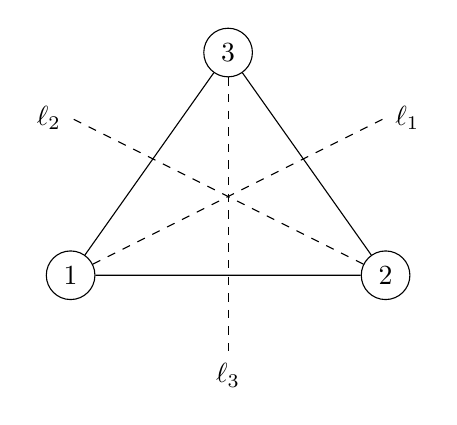
\begin{tikzpicture}
      \node [circle,draw] (1) at (0,0) {1};
      \node [circle,draw] (2) at (4,0) {2};
      \node [circle,draw] (3) at (2,{2*sqrt(2)}) {3};
      \draw (1) -- (2) -- (3) -- (1);
      \draw [dashed] (1) -- (4,2) node [right] {$\ell_1$};
      \draw [dashed] (2) -- (0,2) node [left] {$\ell_2$};
      \draw [dashed] (3) -- (2,-1) node [below] {$\ell_3$};
    \end{tikzpicture}
  \end{minipage}
  \begin{minipage}{3in}
    \begin{tabular}{ll}
      $e=()$ & no action \\
      $r=(123)$ & rotate CCW \\
      $r^{-1}=(132)$ & rotate CW \\
      $f_1=(23)$ & flip about $\ell_1$ \\
      $f_2=(13)$ & flip about $\ell_2$ \\
      $f_3=(12)$ & flip about $\ell_3$ \\
    \end{tabular}
  \end{minipage}

  $r^2=r^{-1}$ \\
  $r^3=(r^{-1})^3=e$ \\
  $f_1=f_1^{-1}$ \\
  $f_2=f_2^{-1}$ \\
  $f_3=f_3^{-1}$ \\
  $f_1^2=f_2^2=f_3^2=e$
\end{example}

\begin{example}[$D_4$]
  \begin{minipage}{3in}
    \begin{tikzpicture}
      \node [circle,draw] (1) at (0,0) {1};
      \node [circle,draw] (2) at (4,0) {2};
      \node [circle,draw] (3) at (4,4) {3};
      \node [circle,draw] (4) at (0,4) {4};
      \draw (1) -- (2) -- (3) -- (4) -- (1);
      \draw [dashed] (5,5) -- (-1,-1) node [left] {$\ell_1$};
      \draw [dashed] (-1,5) -- (5,-1) node [right] {$\ell_2$};
      \draw [dashed] (2,5) -- (2,-1) node [below] {$\ell_3$};
      \draw [dashed] (-1,2) -- (5,2) node [right] {$\ell_4$};
    \end{tikzpicture}
  \end{minipage}
  \begin{minipage}{3in}
    \begin{tabular}{ll}
      $e=()$ & no action \\
      $r_1=(1234)$ & rotate once CCW \\
      $r_2=(13)(24)$ & rotate twice CCW \\
      $r_3=(1432)$ & rotate thrice CCW \\
      $f_1=(24)$ & flip about $\ell_1$ \\
      $f_2=(13)$ & flip about $\ell_2$ \\
      $f_3=(12)(34)$ & flip about $\ell_3$ \\
      $f_4=(14)(23)$ & flip about $\ell_4$ \\
    \end{tabular}
  \end{minipage}
\end{example}
\newpage
$\abs{D_3}=\abs{S_3}=6$

$\abs{D_4}=8$

In general:
\[\abs{D_n}=2n=(n\ \mbox{rotations})+(n\ \mbox{reflections})\]
where:
\[n\ \mbox{reflections}=\begin{cases}
\frac{n}{2}\ \mbox{opposite vertices}+\frac{n}{2}\ \mbox{opposite sides}, &
n\ \mbox{even} \\
n\ \mbox{vertex-opposite side}, & n\ \mbox{odd} \\
\end{cases}\]

Hasse Diagram for $D_4$:

$\begin{array}{c|cccccccc}
  & e & r_1 & r_2 & r_3 & f_1 & f_2 & f_3 & f_4 \\
  \hline
  e & e & r_1 & r_2 & r_3 & f_1 & f_2 & f_3 & f_4 \\
  r_1 & r_1 & r_2 & r_3 & e & f_3 & f_4 & f_2 & f_1 \\
  r_2 & r_2 & r_3 & e & r_1 & f_2 & f_1 & f_4 & f_3 \\
  r_3 & r_3 & e & r_1 & r_2 & f_4 & f_3 & f_1 & f_2 \\
  f_1 & f_1 & f_4 & f_2 & f_3 & e & r_2 & r_3 & r_1 \\
  f_2 & f_2 & f_3 & f_1 & f_4 & r_2 & e & r_1 & r_3 \\
  f_3 & f_3 & f_1 & f_4 & f_2 & r_1 & r_3 & e & r_2 \\
  f_4 & f_4 & f_2 & f_3 & f_1 & r_3 & r_1 & r_2 & e \\
\end{array}$

\begin{minipage}{3in}
  $\cycle{e}=\{e\}$ \\
  $\cycle{r_1}=\cycle{r_3}=\{e,r_1,r_2,r_3\}$ \\
  $\cycle{r_2}=\{e,r_2\}$ \\
  $\cycle{f_1}=\{e,f_1\}$ \\
  $\cycle{f_2}=\{e,f_2\}$ \\
  $\cycle{f_3}=\{e,f_3\}$ \\
  $\cycle{f_4}=\{e,f_4\}$ \\
  $K=\{e, r_2, f_1, f_2\}$ \\
  $K'=\{e, r_2, f_3, f_4\}$ \\
  $D_4=\{e, r_1, r_2, r_3, f_1, f_2, f_3, f_4\}$
\end{minipage}
\begin{minipage}{3in}
  \begin{tikzpicture}
    \node (e) at (3,0) {$e$};
    \node (f1) at (0,2) {$\cycle{f_1},\cycle{f_2}$};
    \node (r2) at (3,2) {$\cycle{r_2}$};
    \node (f3) at (6,2) {$\cycle{f_3},\cycle{f_4}$};
    \node (K) at (0,4) {$K$};
    \node (r1) at (3,4) {$\cycle{r_1}$};
    \node (Kp) at (6,4) {$K'$};
    \node (D4) at (3,6) {$D_4$};
    \draw (e) edge (f1);
    \draw (e) edge (r2);
    \draw (e) edge (f3);
    \draw (f1) edge (K);
    \draw (r2) edge (K);
    \draw (r2) edge (r1);
    \draw (r2) edge (Kp);
    \draw (f3) edge (Kp);
    \draw (K) edge (D4);
    \draw (r1) edge (D4);
    \draw (Kp) edge (D4);
  \end{tikzpicture}
\end{minipage}

\begin{minipage}{3in}
  $\begin{array}{c|cccc}
    & e & r_2 & f_1 & f_2 \\
    \hline
    e & e & r_2 & f_1 & f_2 \\
    r_2 & r_2 & e & f_2 & f_1 \\
    f_1 & f_1 & f_2 & e & r_2 \\
    f_2 & f_2 & f_1 & r_2 & e \\
  \end{array}=K$
\end{minipage}
\begin{minipage}{3in}
  $\begin{array}{c|cccc}
    & e & r_2 & f_3 & f_4 \\
    \hline
    e & e & r_2 & f_3 & f_4 \\
    r_2 & r_2 & e & f_4 & f_3 \\
    f_3 & f_3 & f_4 & e & r_2 \\
    f_4 & f_4 & f_3 & r_2 & e \\
  \end{array}=K'$
\end{minipage}
\end{document}
